\chapter{Восстановление филогенетических деревьев из брейкпоинт графа}

\section{Получение информации из брейкпоинт графа}
Описанные в предыдущей главе методы вычисления редакционного расстояния между геномами можно рассмотреть в ином ключе.
Редакционное расстояние в модели методов основанных на расстояниях \q{стягивает} геномы друг к другу, заставляя их находиться ближе в дереве, то есть,
принимается, что геномы с меньшим редакционным расстоянием находятся в одном поддереве с большей вероятностью.
Иными словами, расстояние дает нам филогенетическую информацию о ветвях в филогенетическом дереве.

В~\cite{xu2010exploring} автор рассматривает несколько оценок редакционного расстояния, включая описанные выше
и вводит концепцию филогенетического паттерна позволяющую применять их к восстановлению деревьев из брейкпоинт графа.
\begin{define}{Филогенетический паттерн} \\
  Филогенетический паттерн $P(\bb{G}, T)$, где $\bb{G}$ - множество геномов,
  а $T$ - топология филогенетического дерева на них - функция, которая для данных входных геномов
  сопоставляет каждой из возможных топологий филогенетического дерева эвристическую оценку так,
  чтобы она была экстремальной только на одной топологии.
\end{define}
Главное свойство данной концепции в том, что имея на руках листовые геномы филогенетического дерева, можно получить всегда только одно возможное дерево.
Тогда если найти филогенетический паттерн, который будет давать экстремальное значение на тех же топологиях,
что и другая оценка $s$ (например, $d_{BP}$), то он будет давать ту же филогенетическую информацию, что и $s$, несмотря на то,
что эту оценку невозможно было бы вычислить, не зная предковых геномов.
Получается, что имея на руках паттерн, то становится возможным получать оптимальное дерево с точки зрения использованной оценки.
Более того, возможно определить множество паттернов, каждый из которых, в общем случае, может давать экстремальное значение на разных топологиях,
для этого для каждого из паттернов необходимо определить тот вес, который он вносит в оценку, для каждого паттерна это будет рассмотрено отдельно.
В~\cite{xu2010exploring} показано, что филогенетические паттерны удобно строить на основе подграфов брейкпоинт графа,
так как зачастую информации (значений оценки) получаемой на основе малых подграфов достаточно для того,
чтобы отличить разные топологии филогенетического дерева и восстановить корректное.
В дальнейшем филогенетический паттерн и подграф на котором он вычисляется будут использоваться взаимозаменяемо.
Рассмотрим предложенный в~\cite{xu2010exploring} паттерн \q{контрастирующая смежность}.
\begin{figure}[H]
  \centering
  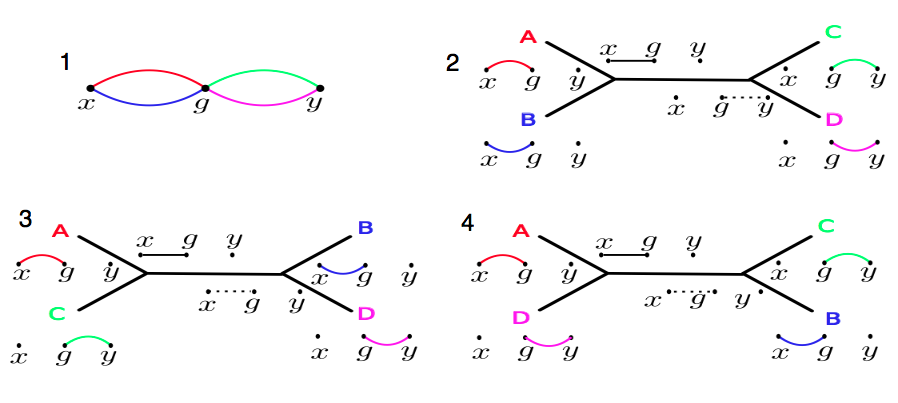
\includegraphics[max width=\linewidth]{fig/2/contrasting_adjacency.png}
  \caption{Контрастирующая смежность.
    1 - подграф, на котором базируется паттерн;
    2 - дерево с топологией $AB|CD$, на котором достигается экстремальное значение $d_{DCJ}$ и $d_{BP}$;
    3, 4 - другие возможные топологии, на которых не достигается экстремальное значение метрик $d_{DCJ}$ и $d_{BP}$}
  \label{fig:contrasting_adjacency}
\end{figure}
Этот паттерн представляет собой подграф брейкпоинт графа из трех вершин, где одна пара соединена двумя ребрами цветов $A$ и $B$, а другая - $C$ и $D$.
Обозначим, что для 4 геномов $A, B, C, D$, $AB|CD$ обозначает, что геномы $A$ и $B$ находятся в одном поддереве, а $C$ и $D$ - в другом.
Тогда для топологии $AB|CD$ можно посчитать расстояние $d (d_{DCJ}, d_{BP})$ как $d(A, B) + d(C, D) + d(I_1, I_2)$,
где $d(\_, \_)$ - функция расстояния между двумя геномами, $I_1, I_2$ - предки в дереве на парах геномов $AB$ и $CD$ соответственно.
Из рисунка~\ref{fig:contrasting_adjacency} можно увидеть, что на топологии $AB|CD$ оценки $d_{BP}$ и $d_{DCJ}$, полученные как указано выше, достигают минимального значения.
Вышеописанный паттерн был обобщен для многих геномов в~\cite{Alekseyev2009} с помощью концепции \textit{простого пути}.
Для того, чтобы ввести эту концепцию введем понятие \textit{альтернирующих мультицветов} на последовательности ребер.
\begin{define}{Альтернирующие мультицвета} \\
  Альтернирующие мультицвета на последовательности ребер $\{e_i\}$ - пара мультицветов $Q$ и $Q'$, таких что
  $\forall i$ если цвет $e_i$ $Q$, то цвет $e_{i + 1}$ - $Q'$ и наоборот, если цвет $e_i$ $Q'$, то цвет $e_{i + 1}$ - $Q$.
\end{define}

\begin{define}{Простой путь} \\
  Простой путь - путь в брейкпоинт графе, состоящий из вершин мультистепени 2 и ребер двух
  мультицветов $Q$ и $Q'$, таких что $Q \cap Q' = \varnothing \land Q \cup Q' = \bb{Q}$,
  где $\bb{Q}$ - множество всех цветов, если путь состоит из последовательности ребер $\{e_i\}$,
  то цвета $Q$ и $Q'$ альтернирующие на $\{e_i\}$.
\end{define}
Оба этих паттерна дают более экстремальную оценку для тех деревьев,
в которых геномы из каждого из альтернирующих мультицветов находятся в одном поддереве.

В брейкпоинт графе один и тот же филогенетический паттерн может встречаться несколько раз и
\q{свидетельствовать} о разном строении филогенетического дерева (более экстремальная оценка достигается на деревьях с разной топологией),
это происходит из-за того, что в паттерн включается только подграф брейкпоинт графа.
Основываясь на предыдущем замечании, можно понять, что информация (\q{свидетельства} о расположении геномов в поддеревьях филогенетического дерева)
извлеченная из брейкпоинт графа будет тем точнее,
чем больше непересекающихся (не использующих одни и те же основания для различия топологий) паттернов будет найдено.
Так становится необходимым искать непересекающиеся филогенетические паттерны в брейкпоинт графах.

Определение паттернов вручную - тяжелый и медленный процесс, потому в данной работе предложен метод их автоматического поиска.
Филогенетический паттерн - это подграф в брейкпоинт графе, раскрашенный в несколько цветов.
Важно заметить два факта:
\begin{enumerate}
  \item Каждый цвет в данном случае необязательно соответствует одному геному, но может соответствовать целой их группе.
  \item Если взять ребра одного цвета из подграфа образующего филогенетический паттерн, то они не будут вершинно пересекаться и образуют паросочетание.
\end{enumerate}

Первый факт важен для получения информации с помощью филогенетических паттернов из брейкпоинт графов для многих геномов,
а второй позволяет перейти к автоматическому поиску филогенетических паттернов.
\begin{figure}[H]
  \centering
  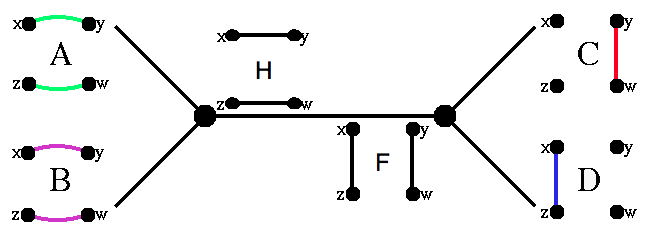
\includegraphics[max width=0.5\linewidth]{fig/2/automatic_pattern_search.png}
  \caption{Схема для перебора паттернов.
    $A, B, C, D$ - конфигурации листовых геномов, каждый из которых является паросочетанием на вершинах брейкпоинт графа.
    $H, F$ - предковые геномы, каждый из которых также является паросочетанием.}
  \label{fig:automatic_pattern_search}
\end{figure}
На рисунке~\ref{fig:automatic_pattern_search} показана схема для перебора паттернов.
Целью перебора является поиск таких 4 конфигураций геномов, на которых обе оценки ($d_{BP}$, $d_{DCJ}$) или одна из них
достигает экстремального значения на одной топологии дерева, но не достигает его на других.
Условие выше выполняется если найдется такая пара конфигураций внутренних вершин,
что на одной из топологий достигается более экстремальное значение оценки, когда на других оно не достигается,
что говорит о том, что найденный набор конфигураций есть филогенетический паттерн.
Ниже представлен алгоритм поиска:
\begin{enumerate}
  \item Выбрать с повторениями 4 паросочетания, как конфигурации геномов.
  \item Для каждой из 3 топологий перебрать паросочетания для внутренних вершин (они тоже являются паросочетаниями).
  \item Выбрать те кортежи из 4 геномов, на которых оценка достигает экстремума.
\end{enumerate}

Важно заметить, что алгоритм выше выполняет перебор, без проверки на уникальность найденных графов, потому необходимо удалить \q{похожие} из них.
Для этого можно определить понятие \textit{изоморфизма паттернов}.
\begin{define}{Изоморфизм паттернов} \\
  Паттерны $A$ и $B$ изоморфны тогда и только тогда, когда существует пара биективных отображений $(f, h)$,
  $f$ - между вершинами паттерна $A$ вершинами паттерна $B$, $h$ - между ребрами паттерна $A$ и ребрами паттерна $B$,
  такая что любые две вершины $u$ и $v$ в $A$ связаны мультимножеством раскрашенных ребер $E$ тогда и только тогда, когда вершины
  $f(u)$ и $f(v)$ связаны $h(E)$.
\end{define}
\vspace{-2em}
\begin{figure}[H]
  \centering
  \minipage{0.25\textwidth}
  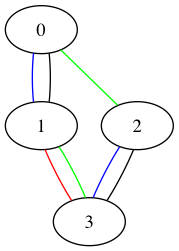
\includegraphics[max width=\linewidth]{fig/2/patterns/similar1.png}
  \endminipage
  \minipage{0.25\textwidth}
    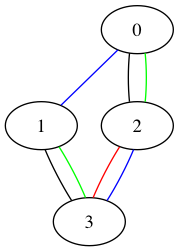
\includegraphics[max width=\linewidth]{fig/2/patterns/similar2.png}
  \endminipage
  \caption{Изоморфные паттерны}
  \label{fig:isomorphic_patterns}
\end{figure}

Таким образом, могут быть найдены все паттерны на любом количестве вершин.
В данной работе удалось провести поиск паттернов на 4 вершинах (перебор на большем числе вершин оказался слишком вычислительно затратным),
в результате него после отсеивания изоморфных паттернов и паттернов, которые учитывались бы в оценках, используемых Wei Xu
(паттерны, содержащие простые пути длины больше 1 или простые циклы) остались следующие паттерны,
показанные на рисунках~\ref{fig:cylinder_pattern} и~\ref{fig:bag_pattern}.
Оба этих паттерна дают более экстремальную оценку для деревьев, в которых цвета,
из которых состоят ребра помеченные звездочкой, находятся в одном поддереве.
\begin{figure}[H]
  \centering
  \minipage{0.25\textwidth}
  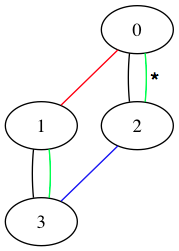
\includegraphics[max width=\linewidth]{fig/2/patterns/cylinder.png}
    \caption{Паттерн \q{цилиндр}}
    \label{fig:cylinder_pattern}
  \endminipage \hspace{1em}
  \minipage{0.25\textwidth}
  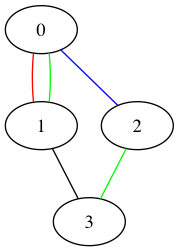
\includegraphics[max width=\linewidth]{fig/2/patterns/bag.png}
    \caption{Паттерн \q{мешок}}
    \label{fig:bag_pattern}
  \endminipage
\end{figure}

\section{Сборка деревьев из разделений}
Смысл использования филогенетических паттернов для восстановления деревьев заключается в том,
чтобы извлечь информацию о устройстве филогенетического дерева из брейкпоинт графа в удобном для восстановления виде.
Так каждая копия филогенетического паттерна найденная в брейкпоинт графе дает информацию о том,
что одна часть геномов находятся ближе друг к другу, а другие - дальше друг от друга в филогенетическом дереве.
Например, если в графе встречается паттерн \q{простой путь} на двух альтернирующих цветах $Q$ и $Q'$, то он \q{свидетельствует},
что геномы из множества $Q$ находятся в одном поддереве, а геномы из множества $Q'$ - в другом, как показано на рисунке~\ref{fig:division}.
\begin{figure}[H]
  \centering
  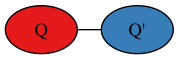
\includegraphics[max width=0.5\linewidth]{fig/2/division.png}
  \caption{Дерево, о котором \q{свидетельствует} простой путь на альтернирующих цветах $Q$ и $Q'$.}
  \label{fig:division}
\end{figure}
Таким образом, механизм филогенетических паттернов позволяет получить из брейкпоинт графа информацию о ветвях филогенетического дерева.
Сформулируем задачу восстановления филогенетического дерева из полученной информации.
Для этого введем понятие \textit{разделения} как единицы информации об устройстве филогенетического дерева.
\begin{define}{Разделение} \\
  Пусть $\bb{Q}$ - множество всех листовых геномов.
  Разделение - пара множеств вида $Q_1|Q_2$, таких, что $Q_1 \subset \bb{Q}$ и $Q_2 \subset \bb{Q}$ и при этом
  $Q_1 \cap Q_2 = \varnothing$ и $Q_1 \cup Q_2 = \bb{Q}$.
\end{define}
Введем обозначения что для разделения вида $D = Q_1|Q_2$, $left(D) = Q_1$, $right(D) = Q_2$.
Также заметим, что для дальнейшего использования разделения $Q_1|Q_2$ и $Q_2|Q_1$,
где $Q_1$, $Q_2$ - подмножества множества всех геномов $\bb{Q}$, идентичны.

Представим каждое вхождение паттерна $P$ в брейкпоинт граф как разделение $Q_1|Q_2$,
если согласно вхождению паттерна $P$ геномы $Q_1$ должны находиться в одном поддереве результирующего филогенетического дерева,
а геномы $Q_2$ - в другом.
Таким образом, если $search(G, P)$ дает набор всех вхождений паттерна $P$ в брейкпоинт граф $G$,
а $toDivision_P(I)$ преобразует вхождение $I$ паттерна $P$ в разделение,
то набор разделений $\bb{D}$ полученный из брейкпоинт графа $G$ и множества паттернов $\bb{P}$ можно выразить как
$\bigcup\nolimits_{P \in \bb{P}} \bigcup\nolimits_{I \in search(G, P)} \{toDivision_P(I)\}$.
В таком случае все разделения считаются одинаково ценными и неясно, как восстановить дерево из них, так как непонятно,
как выбирать из двух противоречащих друг другу разделений то, которое должно войти в результирующее дерево,
потому введем понятие \textit{свидетельства}.
\begin{define}{Свидетельство}\\
  Свидетельство - пара разделения и оценки, указывающей, насколько весома информация о наличии данного разделения в результирующем филогенетического дерева.
\end{define}
Например, простой путь длины $l$ на альтернирующих цветах $Q$ и $Q'$ дает свидетельство в $\floor{\frac{l}{2}}$ единиц и
свидетельство ($Q|Q'$, $\floor{\frac{l}{2}}$).
Далее, сгруппируем все свидетельства с одинаковыми разделениями и сложим их оценки.
Тогда мы получим множество свидетельств $\bb{S} = \{(D, V)\}$, где каждое разделение $D$ встречается не больше одного раза.
Обозначим, что для свидетельства $S = (D, V)$, $D = div(S)$ и $V = value(S)$, а $left(S) = left(div(S))$ и $right(S) = right(div(S))$.
Сформулируем теперь задачу, решение которой даст нам лучшее восстановленное дерево из возможных на основе выделенной филогенетической информации.
\begin{task}{Восстановление филогенетического дерева из свидетельств} \\
  Восстановить филогенетическое дерево с наилучшей оценкой имея на входе набор свидетельств,
  полученных из брейкпоинт графа.
\end{task}

В данной работе будет описано два алгоритма восстановления деревьев из полученных свидетельств:
наивный алгоритм и реализация динамическим программированием.
Для описания алгоритмов введем отношение \textit{непересечения} между двумя разделениями.
\begin{define}{Непересекающиеся разделения} \\
  Два разделения $Q_1|Q_2$ и $R_1|R_2$ \textit{не пересекаются},
  если $Q_1 \cap R_1 = \varnothing \lor Q_1 \cap R_2 = \varnothing $.
\end{define}
\noindent Отношение непересечения симметрично.

\subsection{Наивный алгоритм}
Суть данного алгоритма в том, чтобы перебрать все деревья, о которых \q{свидетельствует} брейкпоинт граф и выбрать из них лучшее.
Отличие данного алгоритма от полного перебора всех деревьев с их оцениванием в том,
что основываясь на свидетельствах полученных из имеющегося брейкпоинт графа часть из них построить невозможно, а поэтому
перебор уменьшится.
Введем понятие \textit{класса непересекающихся разделений}, которое описывает возможное дерево в виде разделений.
\begin{define}{Класс непересекающихся разделений} \\
  Класс непересекающихся разделений $F$ над множеством разделений $\bb{D}$ - подмножество $\bb{D}$,
  в котором любые два разделения не пересекаются между собой.
\end{define}

\noindent Таким же образом определим понятие \textit{класса непересекающихся свидетельств}.
\begin{define}{Класс непересекающихся свидетельств}\\
  Класс непересекающихся свидетельств $H$ над множеством свидетельств $\bb{S}$ - подмножество $\bb{S}$,
  такое что $\forall S \in H: div(S) \in F$,
  где $F$ -  класс непересекающихся разделений над множеством разделений.
\end{define}

\noindent Для класса непересекающихся свидетельств $H$ определим его оценку \\
$value(H) = \sum\nolimits_{S \in H} value(S)$.

\begin{define}{Максимальный класс непересекающихся разделений} \\
  Максимальный класс непересекающихся разделений $F$ на множеством разделений $\bb{D}$ -
  класс непересекающихся разделений над $\bb{D}$, такой что него невозможно добавить новое разделение из $\bb{D}$,
  так чтобы он сохранил свойство непересечения.
\end{define}

\begin{define}{Максимальный класс непересекающихся свидетельств} \\
  Максимальный класс непересекающихся свидетельств $H$ над множеством свидетельств $\bb{S}$ - класс непересекающихся свидетельств $H$,
  такой что $\forall S \in H: div(S) \in F$,
  где $F$ - максимальный класс непересекающихся разделений над множеством разделений.
\end{define}

Заметим, что из исходного множества разделений, в общем случае, можно получить несколько максимальных классов непересекающихся разделений.
\begin{example}
  Рассмотрим случай, что $\bb{D} = \{ AB|CD, AC|BD, A|BCD \}$, где $A, B, C, D$ - геномы.
  В данном случае можно получить максимальные классы непересекающихся разделений
  $H_0 = \{ AB|CD, A|BCD \}$ и $H_1 = \{ AC|BD, A|BCD \}$.
\end{example}
Из этого примера также видно, что разделение может входить в несколько непересекающихся классов разделений одновременно,
что соответствует тому случаю, когда одна ветвь присутствует в разных деревьях.
В~\cite{gusfield1991efficient} показано, что из класса непересекающихся разделений можно построить дерево единственным образом:
для этого необходимо выписать разделения в таблицу $M \times N$, где $M$ - количество разделений в классе, $N$ - количество геномов,
и для каждого генома $G$ и разделения $D = Q_1|Q_2$ записать на их пересечении 1, если $G \in Q_1$ и ноль иначе.

На основе вышеизложенного сформулируем наивный алгоритм:
\begin{enumerate}
  \item Выделить среди свидетельств множество максимальных классов непересекающихся $\bb{C}$
  \item Выбрать лучший по оценке класс из $\bb{C}$
  \item Выделить разделения из свидетельств выбранного класса и собрать из них дерево
\end{enumerate}

\subsection{Реализация динамическим программированием}

Проблемой предыдущего алгоритма являлось то, что он выполнял перебор всех деревьев, о которых \q{свидетельствует} брейкпоинт граф,
в случае многих геномов таких деревьев может быть много, что приведет к тому, что работа алгоритма может занять большое время.
Каждое разделение вида $Q_1|Q_2$ задает ветку в некорневом бинарном дереве с помеченными листьями, иными словами,
делит все множество геномов на два подмножества $Q_1$ и $Q_2$, топология дерева на которых
(расположение геномов из подмножества в филогенетическом дереве) может быть уточнена в дальнейшем другими разделениями.
Из этого следует, что поиск топологий для подмножеств может проводится независимо.
Поиск топологий на подмножестве геномов $G'$ - такая же задача как исходная, но при этом для каждого разделения $D$
из множества разделений (и каждого свидетельства с разделением $D$) из $D$ удаляются все геномы, не присутствующие в $G'$
Теперь, если для любого свидетельства $S$ с разделением вида $Q_1|Q_2$ из некоторого набора $\bb{S}$ известны топологии с наилучшей оценкой,
построенные на множествах геномов $Q_1$ и $Q_2$, то чтобы найти дерево с максимальной оценкой нужно перебрать все свидетельства из $\bb{S}$ и найти то,
оценка которого в сумме с оценками поддеревьев даст наибольшее значение.
Данную логику можно применить также для того, чтобы построить оптимальные деревья для вышеупомянутых пар множеств $Q_1$ и $Q_2$,
составляющих разделения свидетельств.
Таким образом, приходим к задаче динамического программирования для решения которой сформулируем следующий алгоритм:
\begin{enumerate}
  \item Обозначим, что для любого множества $F$ размера $f$, $size(F) = f$.
    Пусть даны множества $\bb{G}$ геномов и $\bb{S}$ имеющихся свидетельств.
    Выпишем построчно набор множеств $\{ SCLevel_i | i = 1..N \}$ в порядке убывания $i$, где $N = size(\bb{G})$,
    a $\forall i, SCLevel_i$ - множество четверок вида $(C, V, V, (null, null))$, таких что $size(C) = i$,
    $\exists S \in \bb{S}: (C = left(S) \lor C = right(S)) \land value(S) = V$ ($null$ обозначает отсутствие значения).
    Компоненты четверки обозначают соответственно: множество геномов, для которого известна топология филогенетического дерева;
    оценку этого множества (оценку свидетельства, в разделении которого это множество присутствует);
    суммарную оценку построенного дерева; пару множеств геномов, на которые делится данное множество геномов.
  \item Начиная с $i = 2$,
    $\forall c = (C, V, CS, SS) \in SCLevel_i$,
    $(C1, V1, CS1, SS1) \in SCLevel_j$,
    $(C2, V2, CS2, SS2) \in SCLevel_k$ обозначим, что $c = (C, V, V + CS1 + CS2, (C1, C2))$,
    если $V + CS1 + CS2$ - максимальное значение при условии  $j = 1..i-1$, $k = i - j$ и $C1 \cup C2 = C \land C1 \cap C2 = \varnothing$
  \item Пусть единственный элемент $SCLevel_N$ имеет вид $(C, V, CS, (C1, C2))$ тогда результирующее дерево можно построить сверху
    вниз для множеств $C1$ и $C2$, после чего объединить результаты корнем.
    Для множеств $C1$ и $C2$ можно выполнить сборку тем же образом, базой для индукции послужит случай,
    когда $C1$ и $C2$ - множества с одним элементом.
\end{enumerate}

\subsection{Примечания к практической реализации}

В первой главе были описаны недостатки существующих решений, которые не позволяли бы им работать с блоками, полученными из геномов со вставками
и удалениями, несобранными геномами или использовать для восстановления информацию об известных поддеревьях восстанавливаемого дерева.
Опишем, как предложенный подход борется с данными проблемами.

Рассмотрим, что происходит с брейкпоинт графом при работе с данными в которых происходили вставки или удаления блоков,
рассмотрим только случай циклических хромосом (в линейных различия будут случаться только в конечных блоках):
при удалении или вставке блока 2 вершины брейкпоинт графа теряют степень $N$ ($N$ - количество геномов), при вставке степень растет,
при удалении - падает.
Для того, чтобы \q{не потерять} структуры графа, зависящие от данных вершин в случае удаления блока выполняется добавление \q{протезного} ребра
необходимого цвета.
Далее свидетельства на графе считаются так же как и раньше, но к результирующим свидетельствам добавляется информация (в форме оценки) о том,
что было добавлено ребро такого цвета.
Данные преобразования приводят к тому, что даже в условиях большого количества вставок или удалений в графе все равно возможно найти
структуры, которые исчезли в процессе эволюции, но при этом также не теряется информация о том, что вставки или удаления произошли.

При работе с несобранными данными возникает проблема того, что при разбиении хромосомы собранного генома теряется одна смежность на каждые
два контига.
Данная потеря не наносит большого вреда, так как обычно при работе с несобранными геномами блоков много больше (зачастую на несколько порядков),
чем контигов, таким образом, потеря связностей из-за несобранности геномов мало влияет на процесс восстановления деревьев.

При работе с реальными данными, возможна ситуация когда из биологических источников доступна информация о расположении геномов в филогенетическом дереве.
Для того, чтобы поддержать работу с известными поддеревьями используется идея того, что любое разделение из известного поддерева должно присутствовать в результирующем.
Для того, чтобы обеспечить выполнение этого требования известное поддерево разбивается на разделения следующим образом:
\begin{enumerate}
  \item Пусть есть известное поддерево $(T, Q) = ((T_1, Q_1), (T_2, Q_2))$, где $T, T_1, T_2$ - бинарные деревья,
    а $Q, Q_1, Q_2$ - множества геномов в содержащиеся, $\bb{Q}$ - множество всех геномов,
    тогда для такого дерева набор разделений $Divisions(T)$ будет выглядеть как
    $\{Q|\bb{Q} \setminus  Q,$ $Q_1|\bb{Q} \setminus Q_1,$ $Q_2|\bb{Q} \setminus Q_2\} \cup Divisions(T_1) \cup Divisions(T_2)$,
    базой для данной индукции будет случай, когда $Q$ - множество из одного генома.
  \item Для каждого из полученных разделений назначаем оценку $\bb{V}=$ \\
    $\sum\nolimits_{S \in \bb{S}} value(S)$, где $\bb{S}$ - множество свидетельств, полученных из брейкпоинт графа.
\end{enumerate}
После таких операций каждое разделение из известного поддерева окажется в результате, так как при сборке любое пересекающееся с ним разделение
принесет меньше веса в оценку результирующего дерева и потому не будет взято.
